% Options for packages loaded elsewhere
\PassOptionsToPackage{unicode}{hyperref}
\PassOptionsToPackage{hyphens}{url}
%
\documentclass[
]{article}
\usepackage{amsmath,amssymb}
\usepackage{iftex}
\ifPDFTeX
  \usepackage[T1]{fontenc}
  \usepackage[utf8]{inputenc}
  \usepackage{textcomp} % provide euro and other symbols
\else % if luatex or xetex
  \usepackage{unicode-math} % this also loads fontspec
  \defaultfontfeatures{Scale=MatchLowercase}
  \defaultfontfeatures[\rmfamily]{Ligatures=TeX,Scale=1}
\fi
\usepackage{lmodern}
\ifPDFTeX\else
  % xetex/luatex font selection
\fi
% Use upquote if available, for straight quotes in verbatim environments
\IfFileExists{upquote.sty}{\usepackage{upquote}}{}
\IfFileExists{microtype.sty}{% use microtype if available
  \usepackage[]{microtype}
  \UseMicrotypeSet[protrusion]{basicmath} % disable protrusion for tt fonts
}{}
\makeatletter
\@ifundefined{KOMAClassName}{% if non-KOMA class
  \IfFileExists{parskip.sty}{%
    \usepackage{parskip}
  }{% else
    \setlength{\parindent}{0pt}
    \setlength{\parskip}{6pt plus 2pt minus 1pt}}
}{% if KOMA class
  \KOMAoptions{parskip=half}}
\makeatother
\usepackage{xcolor}
\usepackage[margin=1in]{geometry}
\usepackage{color}
\usepackage{fancyvrb}
\newcommand{\VerbBar}{|}
\newcommand{\VERB}{\Verb[commandchars=\\\{\}]}
\DefineVerbatimEnvironment{Highlighting}{Verbatim}{commandchars=\\\{\}}
% Add ',fontsize=\small' for more characters per line
\usepackage{framed}
\definecolor{shadecolor}{RGB}{248,248,248}
\newenvironment{Shaded}{\begin{snugshade}}{\end{snugshade}}
\newcommand{\AlertTok}[1]{\textcolor[rgb]{0.94,0.16,0.16}{#1}}
\newcommand{\AnnotationTok}[1]{\textcolor[rgb]{0.56,0.35,0.01}{\textbf{\textit{#1}}}}
\newcommand{\AttributeTok}[1]{\textcolor[rgb]{0.13,0.29,0.53}{#1}}
\newcommand{\BaseNTok}[1]{\textcolor[rgb]{0.00,0.00,0.81}{#1}}
\newcommand{\BuiltInTok}[1]{#1}
\newcommand{\CharTok}[1]{\textcolor[rgb]{0.31,0.60,0.02}{#1}}
\newcommand{\CommentTok}[1]{\textcolor[rgb]{0.56,0.35,0.01}{\textit{#1}}}
\newcommand{\CommentVarTok}[1]{\textcolor[rgb]{0.56,0.35,0.01}{\textbf{\textit{#1}}}}
\newcommand{\ConstantTok}[1]{\textcolor[rgb]{0.56,0.35,0.01}{#1}}
\newcommand{\ControlFlowTok}[1]{\textcolor[rgb]{0.13,0.29,0.53}{\textbf{#1}}}
\newcommand{\DataTypeTok}[1]{\textcolor[rgb]{0.13,0.29,0.53}{#1}}
\newcommand{\DecValTok}[1]{\textcolor[rgb]{0.00,0.00,0.81}{#1}}
\newcommand{\DocumentationTok}[1]{\textcolor[rgb]{0.56,0.35,0.01}{\textbf{\textit{#1}}}}
\newcommand{\ErrorTok}[1]{\textcolor[rgb]{0.64,0.00,0.00}{\textbf{#1}}}
\newcommand{\ExtensionTok}[1]{#1}
\newcommand{\FloatTok}[1]{\textcolor[rgb]{0.00,0.00,0.81}{#1}}
\newcommand{\FunctionTok}[1]{\textcolor[rgb]{0.13,0.29,0.53}{\textbf{#1}}}
\newcommand{\ImportTok}[1]{#1}
\newcommand{\InformationTok}[1]{\textcolor[rgb]{0.56,0.35,0.01}{\textbf{\textit{#1}}}}
\newcommand{\KeywordTok}[1]{\textcolor[rgb]{0.13,0.29,0.53}{\textbf{#1}}}
\newcommand{\NormalTok}[1]{#1}
\newcommand{\OperatorTok}[1]{\textcolor[rgb]{0.81,0.36,0.00}{\textbf{#1}}}
\newcommand{\OtherTok}[1]{\textcolor[rgb]{0.56,0.35,0.01}{#1}}
\newcommand{\PreprocessorTok}[1]{\textcolor[rgb]{0.56,0.35,0.01}{\textit{#1}}}
\newcommand{\RegionMarkerTok}[1]{#1}
\newcommand{\SpecialCharTok}[1]{\textcolor[rgb]{0.81,0.36,0.00}{\textbf{#1}}}
\newcommand{\SpecialStringTok}[1]{\textcolor[rgb]{0.31,0.60,0.02}{#1}}
\newcommand{\StringTok}[1]{\textcolor[rgb]{0.31,0.60,0.02}{#1}}
\newcommand{\VariableTok}[1]{\textcolor[rgb]{0.00,0.00,0.00}{#1}}
\newcommand{\VerbatimStringTok}[1]{\textcolor[rgb]{0.31,0.60,0.02}{#1}}
\newcommand{\WarningTok}[1]{\textcolor[rgb]{0.56,0.35,0.01}{\textbf{\textit{#1}}}}
\usepackage{longtable,booktabs,array}
\usepackage{calc} % for calculating minipage widths
% Correct order of tables after \paragraph or \subparagraph
\usepackage{etoolbox}
\makeatletter
\patchcmd\longtable{\par}{\if@noskipsec\mbox{}\fi\par}{}{}
\makeatother
% Allow footnotes in longtable head/foot
\IfFileExists{footnotehyper.sty}{\usepackage{footnotehyper}}{\usepackage{footnote}}
\makesavenoteenv{longtable}
\usepackage{graphicx}
\makeatletter
\def\maxwidth{\ifdim\Gin@nat@width>\linewidth\linewidth\else\Gin@nat@width\fi}
\def\maxheight{\ifdim\Gin@nat@height>\textheight\textheight\else\Gin@nat@height\fi}
\makeatother
% Scale images if necessary, so that they will not overflow the page
% margins by default, and it is still possible to overwrite the defaults
% using explicit options in \includegraphics[width, height, ...]{}
\setkeys{Gin}{width=\maxwidth,height=\maxheight,keepaspectratio}
% Set default figure placement to htbp
\makeatletter
\def\fps@figure{htbp}
\makeatother
\setlength{\emergencystretch}{3em} % prevent overfull lines
\providecommand{\tightlist}{%
  \setlength{\itemsep}{0pt}\setlength{\parskip}{0pt}}
\setcounter{secnumdepth}{-\maxdimen} % remove section numbering
\ifLuaTeX
  \usepackage{selnolig}  % disable illegal ligatures
\fi
\usepackage{bookmark}
\IfFileExists{xurl.sty}{\usepackage{xurl}}{} % add URL line breaks if available
\urlstyle{same}
\hypersetup{
  hidelinks,
  pdfcreator={LaTeX via pandoc}}

\author{}
\date{\vspace{-2.5em}}

\begin{document}

\section{Introduction}\label{introduction}

This document outlines the progress of my masters thesis. The objective
of this project is to assess biodiversity in the Arctic Tundra using
spectral species analysis.The key tasks include:

\begin{itemize}
\tightlist
\item
  Data collection and pre-processing
\item
  Calculating relative abundance and variance for each species.
\item
  Identifying significant species based on defined thresholds.
\item
  Use the R-package BiodivmapR package to calculate \(\alpha\) and
  \(\beta\)- diversity
\end{itemize}

\begin{center}\rule{0.5\linewidth}{0.5pt}\end{center}

\section{Data Preparation and Code}\label{data-preparation-and-code}

The following steps were taken to prepare the data and perform the
analysis:

\subsection{Define project parameters}\label{define-project-parameters}

All of the scripts access the information set in the parameter document
\href{https://github.com/patrickangst/UWW200_Master_Thesis_public/blob/main/MasterThesisRCode/00_Project_Parameter.R}{00\_Project\_Parameter.R}

\begin{Shaded}
\begin{Highlighting}[]

\CommentTok{\# filename of the raw hyperspectral image}
\NormalTok{file\_name }\OtherTok{\textless{}{-}} \StringTok{\textquotesingle{}ang20190712t231624\_rfl\_v2v2\_img\textquotesingle{}}

\CommentTok{\# definition of the subzone (c, d or e)}
\NormalTok{subzone }\OtherTok{\textless{}{-}} \StringTok{\textquotesingle{}c\textquotesingle{}}
\NormalTok{file\_name\_rectified }\OtherTok{\textless{}{-}} \FunctionTok{paste0}\NormalTok{(file\_name,}\StringTok{\textquotesingle{}\_rectified\textquotesingle{}}\NormalTok{)}

\CommentTok{\# definition of the thresholdes for the mask creation}
\NormalTok{ndwi\_threshold }\OtherTok{\textless{}{-}} \FloatTok{0.1}
\NormalTok{ndvi\_threshold }\OtherTok{\textless{}{-}} \FloatTok{0.3}
\NormalTok{savi\_threshold }\OtherTok{\textless{}{-}} \FloatTok{0.2}
\NormalTok{savi\_L }\OtherTok{\textless{}{-}} \FloatTok{0.5}

\CommentTok{\#create additional variables for the masks}
\NormalTok{mask\_name\_suffix }\OtherTok{\textless{}{-}} \FunctionTok{gsub}\NormalTok{(}\StringTok{"}\SpecialCharTok{\textbackslash{}\textbackslash{}}\StringTok{."}\NormalTok{, }\StringTok{""}\NormalTok{, savi\_threshold)}
\NormalTok{mask\_name }\OtherTok{\textless{}{-}} \FunctionTok{paste0}\NormalTok{(file\_name\_rectified,}\StringTok{\textquotesingle{}\_savi\_mask\_\textquotesingle{}}\NormalTok{,mask\_name\_suffix)}

\CommentTok{\# get the base path of the project}
\NormalTok{base\_path }\OtherTok{\textless{}{-}} \FunctionTok{getwd}\NormalTok{()}
\end{Highlighting}
\end{Shaded}

\subsection{Create an RGB image of the
flightstrip}\label{create-an-rgb-image-of-the-flightstrip}

For quick analysis the RGB bands are extracted from the hyperspectal
image and saved as a GeoTiff file
\href{https://github.com/patrickangst/UWW200_Master_Thesis_public/blob/main/MasterThesisRCode/01_Create_RGB.R}{01\_Create\_RGB.R}

\begin{Shaded}
\begin{Highlighting}[]
\CommentTok{\# Clear workspace and graphics}
\FunctionTok{rm}\NormalTok{(}\AttributeTok{list =} \FunctionTok{ls}\NormalTok{())}
\FunctionTok{graphics.off}\NormalTok{()}

\CommentTok{\# Define parameter script}
\FunctionTok{source}\NormalTok{(}\StringTok{\textquotesingle{}00\_Project\_Parameter.R\textquotesingle{}}\NormalTok{)}


\NormalTok{raw\_image\_file\_path }\OtherTok{\textless{}{-}} \FunctionTok{paste0}\NormalTok{(base\_path,}\StringTok{\textquotesingle{}/data/hs\_raw\_image/\textquotesingle{}}\NormalTok{,file\_name)}
\NormalTok{rgb\_image\_file\_path }\OtherTok{\textless{}{-}} \FunctionTok{paste0}\NormalTok{(base\_path,}\StringTok{\textquotesingle{}/data/rgb/\textquotesingle{}}\NormalTok{,file\_name,}\StringTok{\textquotesingle{}\_rgb.tif\textquotesingle{}}\NormalTok{)}

\CommentTok{\# Define the bands you want to select}
\NormalTok{bandselection }\OtherTok{\textless{}{-}} \StringTok{"{-}b 59 {-}b 34 {-}b 20"}

\CommentTok{\# GDAL translate command to extract the specified bands and create a new image}
\NormalTok{gdal\_translate\_command }\OtherTok{\textless{}{-}} \FunctionTok{sprintf}\NormalTok{(}\StringTok{"gdal\_translate \%s {-}of GTiff \%s \%s"}\NormalTok{, bandselection, raw\_image\_file\_path, rgb\_image\_file\_path)}

\CommentTok{\# Execute the GDAL translate command}
\FunctionTok{system}\NormalTok{(gdal\_translate\_command)}

\CommentTok{\# Check if the output file was created successfully}
\ControlFlowTok{if}\NormalTok{ (}\FunctionTok{file.exists}\NormalTok{(rgb\_image\_file\_path)) \{}
  \FunctionTok{cat}\NormalTok{(}\StringTok{"Output file created successfully:"}\NormalTok{, rgb\_image\_file\_path, }\StringTok{"}\SpecialCharTok{\textbackslash{}n}\StringTok{"}\NormalTok{)}

  \CommentTok{\# GDAL edit command to set color interpretation for each band}
\NormalTok{  gdal\_edit\_command }\OtherTok{\textless{}{-}} \FunctionTok{sprintf}\NormalTok{(}\StringTok{"gdal\_edit.py {-}colorinterp\_1 Red {-}colorinterp\_2 Green {-}colorinterp\_3 Blue \%s"}\NormalTok{, rgb\_image\_file\_path)}

  \CommentTok{\# Execute the GDAL edit command}
  \FunctionTok{system}\NormalTok{(gdal\_edit\_command)}

  \CommentTok{\# Confirm that color interpretation was set successfully}
  \FunctionTok{cat}\NormalTok{(}\StringTok{"Color interpretation set to RGB for each band in"}\NormalTok{, rgb\_image\_file\_path, }\StringTok{"}\SpecialCharTok{\textbackslash{}n}\StringTok{"}\NormalTok{)}

\NormalTok{\} }\ControlFlowTok{else}\NormalTok{ \{}
  \FunctionTok{cat}\NormalTok{(}\StringTok{"Failed to create output file.}\SpecialCharTok{\textbackslash{}n}\StringTok{"}\NormalTok{)}
\NormalTok{\}}
\end{Highlighting}
\end{Shaded}

\subsection{Image reactification}\label{image-reactification}

To follow the format set by the BiodivmapR package, the raw
hyperspectral image has to be transformed. Using
\href{https://gdal.org/en/latest/programs/gdalwarp.html}{gdalwarp}, the
no-data values -9999 have to be replaced with 0 and the image
organization has to be set to
\href{https://desktop.arcgis.com/en/arcmap/latest/manage-data/raster-and-images/bil-bip-and-bsq-raster-files.htm}{BIL}
(Band interleaved by line).
\href{https://github.com/patrickangst/UWW200_Master_Thesis_public/blob/main/MasterThesisRCode/02_Rectify_Image.R}{02\_Rectify\_Image.R}

\begin{Shaded}
\begin{Highlighting}[]
\CommentTok{\# Clear workspace and graphics}
\FunctionTok{rm}\NormalTok{(}\AttributeTok{list =} \FunctionTok{ls}\NormalTok{())}
\FunctionTok{graphics.off}\NormalTok{()}

\FunctionTok{library}\NormalTok{(sf)}
\FunctionTok{library}\NormalTok{(terra)}

\CommentTok{\# Define parameter script}
\FunctionTok{source}\NormalTok{(}\StringTok{\textquotesingle{}00\_Project\_Parameter.R\textquotesingle{}}\NormalTok{)}

\CommentTok{\#boundary\_file\_path \textless{}{-} paste0(base\_path, \textquotesingle{}/cutline/crop\_large/crop\_large.shp\textquotesingle{})}
\NormalTok{raw\_image\_file\_path }\OtherTok{\textless{}{-}} \FunctionTok{paste0}\NormalTok{(base\_path, }\StringTok{\textquotesingle{}/data/hs\_raw\_image/\textquotesingle{}}\NormalTok{, file\_name)}
\NormalTok{rectified\_image\_file\_path }\OtherTok{\textless{}{-}} \FunctionTok{paste0}\NormalTok{(base\_path, }\StringTok{\textquotesingle{}/data/rectified/\textquotesingle{}}\NormalTok{, file\_name\_rectified)}
\NormalTok{rectified\_hdr\_file\_path }\OtherTok{\textless{}{-}} \FunctionTok{paste0}\NormalTok{(rectified\_image\_file\_path, }\StringTok{\textquotesingle{}.hdr\textquotesingle{}}\NormalTok{)}

\NormalTok{target\_srs }\OtherTok{\textless{}{-}} \StringTok{"EPSG:32604"}  \CommentTok{\# Define target CRS}

\NormalTok{gdal\_command\_rectify }\OtherTok{\textless{}{-}} \FunctionTok{sprintf}\NormalTok{(}
  \StringTok{"gdalwarp {-}of ENVI {-}co INTERLEAVE=BIL {-}srcnodata {-}9999 {-}dstnodata 0 \%s \%s"}\NormalTok{,}
\NormalTok{  raw\_image\_file\_path,}
\NormalTok{  rectified\_image\_file\_path}
\NormalTok{)}

\CommentTok{\# Print the command to check if it\textquotesingle{}s correctly formed}
\FunctionTok{print}\NormalTok{(gdal\_command\_rectify)}

\CommentTok{\# Execute the command in R}
\FunctionTok{system}\NormalTok{(gdal\_command\_rectify)}

\CommentTok{\# ===============================================================================}
\CommentTok{\# Define wavelength information to add to .hdr file}
\NormalTok{wavelength\_values }\OtherTok{\textless{}{-}} \FunctionTok{c}\NormalTok{(}
  \FloatTok{376.719576}\NormalTok{ ,}
  \FloatTok{381.729576}\NormalTok{ ,}
\NormalTok{  ...}
\NormalTok{)}

\NormalTok{wavelength\_units }\OtherTok{\textless{}{-}} \StringTok{"Nanometers"}
\NormalTok{wavelength\_line }\OtherTok{\textless{}{-}} \FunctionTok{paste}\NormalTok{(}\StringTok{"wavelength = \{"}\NormalTok{, }\FunctionTok{paste}\NormalTok{(wavelength\_values, }\AttributeTok{collapse =} \StringTok{" , "}\NormalTok{), }\StringTok{"\}"}\NormalTok{)}
\NormalTok{units\_line }\OtherTok{\textless{}{-}} \FunctionTok{paste}\NormalTok{(}\StringTok{"wavelength units ="}\NormalTok{, wavelength\_units)}

\CommentTok{\# ===============================================================================}
\CommentTok{\# Append wavelength information to the .hdr file}
\ControlFlowTok{if}\NormalTok{ (}\FunctionTok{file.exists}\NormalTok{(rectified\_hdr\_file\_path)) \{}
  \CommentTok{\# Read the existing content of the .hdr file}
\NormalTok{  hdr\_content }\OtherTok{\textless{}{-}} \FunctionTok{readLines}\NormalTok{(rectified\_hdr\_file\_path)}

  \CommentTok{\# Append the wavelength information at the end of the file}
\NormalTok{  hdr\_content }\OtherTok{\textless{}{-}} \FunctionTok{c}\NormalTok{(hdr\_content, units\_line, wavelength\_line)}

  \CommentTok{\# Write the updated content back to the .hdr file}
  \FunctionTok{writeLines}\NormalTok{(hdr\_content, rectified\_hdr\_file\_path)}

  \FunctionTok{cat}\NormalTok{(}\StringTok{"Wavelength information successfully added to the .hdr file.}\SpecialCharTok{\textbackslash{}n}\StringTok{"}\NormalTok{)}
\NormalTok{\} }\ControlFlowTok{else}\NormalTok{ \{}
  \FunctionTok{cat}\NormalTok{(}\StringTok{"Error: The .hdr file does not exist. Check the file path.}\SpecialCharTok{\textbackslash{}n}\StringTok{"}\NormalTok{)}
\NormalTok{\}}

\FunctionTok{print}\NormalTok{(}\FunctionTok{paste0}\NormalTok{(}\StringTok{\textquotesingle{}Rectification done for \textquotesingle{}}\NormalTok{, file\_name))}
\end{Highlighting}
\end{Shaded}

\subsection{Mask creation}\label{mask-creation}

Since not all pixels have to be processed, only the ``valid'' have to be
selected. For this purpose, a
\href{https://www.usgs.gov/landsat-missions/landsat-soil-adjusted-vegetation-index}{Soil
Adjusted Vegetation Index (SAVI)} mask is created.
\href{https://github.com/patrickangst/UWW200_Master_Thesis_public/blob/main/MasterThesisRCode/03_Create_MASK.R}{03\_Create\_MASK.R}

\begin{Shaded}
\begin{Highlighting}[]
\CommentTok{\# clean environment}
\FunctionTok{rm}\NormalTok{(}\AttributeTok{list=}\FunctionTok{ls}\NormalTok{(}\AttributeTok{all=}\ConstantTok{TRUE}\NormalTok{));}\FunctionTok{gc}\NormalTok{()}
\FunctionTok{graphics.off}\NormalTok{()}

\FunctionTok{library}\NormalTok{(terra)}

\CommentTok{\# Define parameter script}
\FunctionTok{source}\NormalTok{(}\StringTok{\textquotesingle{}00\_Project\_Parameter.R\textquotesingle{}}\NormalTok{)}

\NormalTok{file\_name }\OtherTok{\textless{}{-}}\NormalTok{ file\_name\_rectified}
\NormalTok{cell }\OtherTok{\textless{}{-}} \FunctionTok{paste0}\NormalTok{(base\_path,}\StringTok{\textquotesingle{}/data/rectified/\textquotesingle{}}\NormalTok{,file\_name)}
\NormalTok{tile }\OtherTok{\textless{}{-}} \FunctionTok{rast}\NormalTok{(}\FunctionTok{file.path}\NormalTok{(cell))}

\CommentTok{\# Plot the RGB image for a quick check}
\FunctionTok{plot}\NormalTok{(}\FunctionTok{ext}\NormalTok{(tile))}
\FunctionTok{plotRGB}\NormalTok{(tile, }\AttributeTok{add=}\NormalTok{T, }\AttributeTok{r=}\DecValTok{54}\NormalTok{, }\AttributeTok{g=}\DecValTok{36}\NormalTok{, }\AttributeTok{b=}\DecValTok{20}\NormalTok{, }\AttributeTok{stretch=}\StringTok{"lin"}\NormalTok{)}


\CommentTok{\# Calculate the mean of a few values of the near infrared bands (used for NDWI and SAVI)}
\NormalTok{NIR\_average }\OtherTok{\textless{}{-}} \FunctionTok{mean}\NormalTok{(tile[[}\FunctionTok{c}\NormalTok{(}\DecValTok{86}\NormalTok{, }\DecValTok{87}\NormalTok{, }\DecValTok{88}\NormalTok{, }\DecValTok{89}\NormalTok{, }\DecValTok{90}\NormalTok{, }\DecValTok{91}\NormalTok{, }\DecValTok{92}\NormalTok{, }\DecValTok{93}\NormalTok{, }\DecValTok{94}\NormalTok{, }\DecValTok{95}\NormalTok{, }\DecValTok{96}\NormalTok{, }\DecValTok{97}\NormalTok{, }\DecValTok{98}\NormalTok{, }\DecValTok{99}\NormalTok{, }\DecValTok{100}\NormalTok{, }\DecValTok{101}\NormalTok{, }\DecValTok{102}\NormalTok{, }\DecValTok{103}\NormalTok{, }\DecValTok{104}\NormalTok{, }\DecValTok{105}\NormalTok{)]])}
\CommentTok{\# Calculate green band averages (used for NDWI)}
\NormalTok{green\_average }\OtherTok{\textless{}{-}} \FunctionTok{mean}\NormalTok{(tile[[}\FunctionTok{c}\NormalTok{(}\DecValTok{26}\NormalTok{, }\DecValTok{27}\NormalTok{, }\DecValTok{28}\NormalTok{,}\DecValTok{29}\NormalTok{,}\DecValTok{30}\NormalTok{,}\DecValTok{31}\NormalTok{,}\DecValTok{32}\NormalTok{,}\DecValTok{33}\NormalTok{,}\DecValTok{34}\NormalTok{,}\DecValTok{35}\NormalTok{,}\DecValTok{36}\NormalTok{,}\DecValTok{37}\NormalTok{,}\DecValTok{38}\NormalTok{,}\DecValTok{39}\NormalTok{,}\DecValTok{40}\NormalTok{,}\DecValTok{41}\NormalTok{,}\DecValTok{42}\NormalTok{,}\DecValTok{43}\NormalTok{,}\DecValTok{44}\NormalTok{,}\DecValTok{45}\NormalTok{)]])}
\CommentTok{\# Calculate red band averages (used for SAVI)}
\NormalTok{red\_average }\OtherTok{\textless{}{-}} \FunctionTok{mean}\NormalTok{(tile[[}\FunctionTok{c}\NormalTok{(}\DecValTok{56}\NormalTok{, }\DecValTok{57}\NormalTok{, }\DecValTok{58}\NormalTok{, }\DecValTok{59}\NormalTok{, }\DecValTok{60}\NormalTok{, }\DecValTok{61}\NormalTok{, }\DecValTok{62}\NormalTok{, }\DecValTok{63}\NormalTok{, }\DecValTok{64}\NormalTok{, }\DecValTok{65}\NormalTok{)]])}

\CommentTok{\# Plot histogram of the distribution of the values}
\FunctionTok{hist}\NormalTok{(NIR\_average, }\AttributeTok{breaks =} \FunctionTok{seq}\NormalTok{(terra}\SpecialCharTok{::}\FunctionTok{minmax}\NormalTok{(NIR\_average)[}\DecValTok{1}\NormalTok{], terra}\SpecialCharTok{::}\FunctionTok{minmax}\NormalTok{(NIR\_average)[}\DecValTok{2}\NormalTok{] }\SpecialCharTok{+} \FloatTok{0.05}\NormalTok{, }\AttributeTok{by =} \FloatTok{0.01}\NormalTok{),}
     \AttributeTok{main =} \StringTok{"Histogram of NIR average"}\NormalTok{, }\AttributeTok{xlab =} \StringTok{"NIR\_average"}\NormalTok{)}


\DocumentationTok{\#\#\#\#\#\#\#\#\#\#\#\#\#\#\#\#\#\#\#\#\#\#\#\#\#\#\#\#\#\#\#\#\#\#\#\#\#\#\#\#\#\#\#\#\#\#\#\#\#\#\#\#\#\#\#\#\#\#\#\#\#\#\#\#\#\#\#\#\#\#\#\#\#\#\#\#\#\#\#\#}
\CommentTok{\# Create NDWI Mask NDWI = (Red {-} NIR) / (Red + NIR)}
\DocumentationTok{\#\#\#\#\#\#\#\#\#\#\#\#\#\#\#\#\#\#\#\#\#\#\#\#\#\#\#\#\#\#\#\#\#\#\#\#\#\#\#\#\#\#\#\#\#\#\#\#\#\#\#\#\#\#\#\#\#\#\#\#\#\#\#\#\#\#\#\#\#\#\#\#\#\#\#\#\#\#\#\#}

\CommentTok{\# Calculate the NDWI}
\NormalTok{NDWI }\OtherTok{\textless{}{-}}\NormalTok{ (green\_average}\SpecialCharTok{{-}}\NormalTok{NIR\_average)}\SpecialCharTok{/}\NormalTok{(green\_average}\SpecialCharTok{+}\NormalTok{NIR\_average)}

\CommentTok{\# Plot histogram of the value distribution}
\FunctionTok{hist}\NormalTok{(NDWI, }\AttributeTok{breaks =} \FunctionTok{seq}\NormalTok{(terra}\SpecialCharTok{::}\FunctionTok{minmax}\NormalTok{(NDWI)[}\DecValTok{1}\NormalTok{], terra}\SpecialCharTok{::}\FunctionTok{minmax}\NormalTok{(NDWI)[}\DecValTok{2}\NormalTok{] }\SpecialCharTok{+} \FloatTok{0.05}\NormalTok{, }\AttributeTok{by =} \FloatTok{0.01}\NormalTok{),}
     \AttributeTok{main =} \StringTok{"Histogram of NDWI"}\NormalTok{, }\AttributeTok{xlab =} \StringTok{"NDWI"}\NormalTok{)}

\CommentTok{\# Create the NDWI mask (binary values) with a threshold of 0.1}
\CommentTok{\#ndwi\_threshold \textless{}{-} ndwi\_threshold}
\NormalTok{ndwi\_mask }\OtherTok{\textless{}{-}} \FunctionTok{ifel}\NormalTok{(NDWI}\SpecialCharTok{\textgreater{}}\NormalTok{ndwi\_threshold, }\DecValTok{0}\NormalTok{, }\DecValTok{1}\NormalTok{)}

\CommentTok{\# Plot the NDWI mask}
\FunctionTok{plot}\NormalTok{(ndwi\_mask, }\AttributeTok{main =} \StringTok{"NDWI Mask"}\NormalTok{)}

\CommentTok{\# Set value 0 to NA to exclude the unwanted pixels}
\NormalTok{ndwi\_mask }\OtherTok{\textless{}{-}} \FunctionTok{ifel}\NormalTok{(ndwi\_mask}\SpecialCharTok{==}\DecValTok{0}\NormalTok{, }\ConstantTok{NA}\NormalTok{, }\DecValTok{1}\NormalTok{)}

\CommentTok{\# If desired, save the NDWI mask to a file}
\NormalTok{ndwi\_threshold\_modified }\OtherTok{\textless{}{-}} \FunctionTok{gsub}\NormalTok{(}\StringTok{"}\SpecialCharTok{\textbackslash{}\textbackslash{}}\StringTok{."}\NormalTok{, }\StringTok{""}\NormalTok{, ndwi\_threshold)}

\NormalTok{ndwi\_filename }\OtherTok{\textless{}{-}} \FunctionTok{paste0}\NormalTok{(base\_path,}\StringTok{"/mask/"}\NormalTok{,file\_name\_rectified,}\StringTok{"\_ndwi\_mask\_"}\NormalTok{,ndwi\_threshold\_modified)}
\FunctionTok{writeRaster}\NormalTok{(ndwi\_mask, }\AttributeTok{filename =} \FunctionTok{file.path}\NormalTok{(ndwi\_filename),}
            \AttributeTok{filetype =} \StringTok{"ENVI"}\NormalTok{,}
            \AttributeTok{gdal =} \StringTok{"INTERLEAVE=BSQ"}\NormalTok{,}
            \AttributeTok{overwrite =} \ConstantTok{TRUE}\NormalTok{,}
            \AttributeTok{datatype =} \StringTok{"INT1U"}\NormalTok{)}

\DocumentationTok{\#\#\#\#\#\#\#\#\#\#\#\#\#\#\#\#\#\#\#\#\#\#\#\#\#\#\#\#\#\#\#\#\#\#\#\#\#\#\#\#\#\#\#\#\#\#\#\#\#\#\#\#\#\#\#\#\#\#\#\#\#\#\#\#\#\#\#\#\#\#\#\#\#\#\#\#\#\#\#\#}
\CommentTok{\# Create NDVI Mask NDVI = (NIR {-} Red) / (NIR + Red)}
\DocumentationTok{\#\#\#\#\#\#\#\#\#\#\#\#\#\#\#\#\#\#\#\#\#\#\#\#\#\#\#\#\#\#\#\#\#\#\#\#\#\#\#\#\#\#\#\#\#\#\#\#\#\#\#\#\#\#\#\#\#\#\#\#\#\#\#\#\#\#\#\#\#\#\#\#\#\#\#\#\#\#\#\#}

\CommentTok{\# Calculate the NDVI}
\NormalTok{NDVI }\OtherTok{\textless{}{-}}\NormalTok{ (NIR\_average}\SpecialCharTok{{-}}\NormalTok{red\_average)}\SpecialCharTok{/}\NormalTok{(NIR\_average}\SpecialCharTok{+}\NormalTok{red\_average)}

\CommentTok{\# Plot histogram of the value distribution}
\FunctionTok{hist}\NormalTok{(NDVI, }\AttributeTok{breaks =} \FunctionTok{seq}\NormalTok{(terra}\SpecialCharTok{::}\FunctionTok{minmax}\NormalTok{(NDVI)[}\DecValTok{1}\NormalTok{], terra}\SpecialCharTok{::}\FunctionTok{minmax}\NormalTok{(NDVI)[}\DecValTok{2}\NormalTok{] }\SpecialCharTok{+} \FloatTok{0.05}\NormalTok{, }\AttributeTok{by =} \FloatTok{0.01}\NormalTok{),}
     \AttributeTok{main =} \StringTok{"Histogram of NDVI"}\NormalTok{, }\AttributeTok{xlab =} \StringTok{"NDVI"}\NormalTok{)}

\CommentTok{\# Create the NDVI mask (binary values) with a threshold of 0.1}
\CommentTok{\#ndvi\_threshold \textless{}{-} 0.3}
\NormalTok{ndvi\_mask }\OtherTok{\textless{}{-}} \FunctionTok{ifel}\NormalTok{(NDVI}\SpecialCharTok{\textgreater{}}\NormalTok{ndvi\_threshold, }\DecValTok{1}\NormalTok{, }\DecValTok{0}\NormalTok{)}

\CommentTok{\# Plot the NDVI mask}
\FunctionTok{plot}\NormalTok{(ndvi\_mask, }\AttributeTok{main =} \StringTok{"NDVI Mask"}\NormalTok{)}

\CommentTok{\# Set value 0 to NA to exclude the unwanted pixels}
\NormalTok{ndvi\_mask }\OtherTok{\textless{}{-}} \FunctionTok{ifel}\NormalTok{(ndvi\_mask}\SpecialCharTok{==}\DecValTok{0}\NormalTok{, }\ConstantTok{NA}\NormalTok{, }\DecValTok{1}\NormalTok{)}

\CommentTok{\# If desired, save the NDVI mask to a file}
\NormalTok{ndvi\_threshold\_modified }\OtherTok{\textless{}{-}} \FunctionTok{gsub}\NormalTok{(}\StringTok{"}\SpecialCharTok{\textbackslash{}\textbackslash{}}\StringTok{."}\NormalTok{, }\StringTok{""}\NormalTok{, ndvi\_threshold)}

\NormalTok{ndvi\_filename }\OtherTok{\textless{}{-}} \FunctionTok{paste0}\NormalTok{(base\_path,}\StringTok{"/mask/"}\NormalTok{,file\_name\_rectified,}\StringTok{"\_ndvi\_mask\_"}\NormalTok{,ndvi\_threshold\_modified)}
\FunctionTok{writeRaster}\NormalTok{(ndvi\_mask, }\AttributeTok{filename =} \FunctionTok{file.path}\NormalTok{(ndvi\_filename),}
            \AttributeTok{filetype =} \StringTok{"ENVI"}\NormalTok{,}
            \AttributeTok{gdal =} \StringTok{"INTERLEAVE=BSQ"}\NormalTok{,}
            \AttributeTok{overwrite =} \ConstantTok{TRUE}\NormalTok{,}
            \AttributeTok{datatype =} \StringTok{"INT1U"}\NormalTok{)}

\DocumentationTok{\#\#\#\#\#\#\#\#\#\#\#\#\#\#\#\#\#\#\#\#\#\#\#\#\#\#\#\#\#\#\#\#\#\#\#\#\#\#\#\#\#\#\#\#\#\#\#\#\#\#\#\#\#\#\#\#\#\#\#\#\#\#\#\#\#\#\#\#\#\#\#\#\#\#\#\#\#\#\#\#}
\CommentTok{\# Create SAVI Mask SAVI = ((NIR {-} Red) / (NIR + Red + L)) * (1 + L)}
\DocumentationTok{\#\#\#\#\#\#\#\#\#\#\#\#\#\#\#\#\#\#\#\#\#\#\#\#\#\#\#\#\#\#\#\#\#\#\#\#\#\#\#\#\#\#\#\#\#\#\#\#\#\#\#\#\#\#\#\#\#\#\#\#\#\#\#\#\#\#\#\#\#\#\#\#\#\#\#\#\#\#\#\#}

\CommentTok{\# Set the L parameter for SAVI}
\NormalTok{L }\OtherTok{\textless{}{-}}\NormalTok{ savi\_L}

\CommentTok{\# Calculate the SAVI}
\NormalTok{SAVI }\OtherTok{\textless{}{-}}\NormalTok{ ((NIR\_average }\SpecialCharTok{{-}}\NormalTok{ red\_average) }\SpecialCharTok{*}\NormalTok{ (}\DecValTok{1} \SpecialCharTok{+}\NormalTok{ L)) }\SpecialCharTok{/}\NormalTok{ (NIR\_average }\SpecialCharTok{+}\NormalTok{ red\_average }\SpecialCharTok{+}\NormalTok{ L)}

\CommentTok{\# Plot a histogram of the SAVI values to inspect the distribution}
\FunctionTok{hist}\NormalTok{(SAVI, }\AttributeTok{breaks =} \FunctionTok{seq}\NormalTok{(terra}\SpecialCharTok{::}\FunctionTok{minmax}\NormalTok{(SAVI)[}\DecValTok{1}\NormalTok{], terra}\SpecialCharTok{::}\FunctionTok{minmax}\NormalTok{(SAVI)[}\DecValTok{2}\NormalTok{] }\SpecialCharTok{+} \FloatTok{0.05}\NormalTok{, }\AttributeTok{by =} \FloatTok{0.01}\NormalTok{),}
     \AttributeTok{main =} \StringTok{"Histogram of SAVI"}\NormalTok{, }\AttributeTok{xlab =} \StringTok{"SAVI"}\NormalTok{)}

\CommentTok{\# Create a SAVI mask (e.g., thresholding SAVI to identify vegetation)}
\CommentTok{\# This threshold can be adjusted based on your analysis needs}
\CommentTok{\#savi\_threshold \textless{}{-} 0.2}

\NormalTok{savi\_mask }\OtherTok{\textless{}{-}} \FunctionTok{ifel}\NormalTok{(SAVI }\SpecialCharTok{\textgreater{}}\NormalTok{ savi\_threshold, }\DecValTok{1}\NormalTok{, }\DecValTok{0}\NormalTok{)  }\CommentTok{\# Here, 0.2 is an example threshold}

\CommentTok{\# Plot the SAVI mask}
\FunctionTok{plot}\NormalTok{(savi\_mask, }\AttributeTok{main =} \StringTok{"SAVI Mask"}\NormalTok{)}

\CommentTok{\# Set value 0 to NA to exclude the unwanted pixels}
\NormalTok{savi\_mask }\OtherTok{\textless{}{-}} \FunctionTok{ifel}\NormalTok{(savi\_mask}\SpecialCharTok{==}\DecValTok{0}\NormalTok{, }\ConstantTok{NA}\NormalTok{, }\DecValTok{1}\NormalTok{)}

\CommentTok{\# If desired, save the SAVI mask to a file}
\NormalTok{savi\_threshold\_modified }\OtherTok{\textless{}{-}} \FunctionTok{gsub}\NormalTok{(}\StringTok{"}\SpecialCharTok{\textbackslash{}\textbackslash{}}\StringTok{."}\NormalTok{, }\StringTok{""}\NormalTok{, savi\_threshold)}

\NormalTok{savi\_filename }\OtherTok{\textless{}{-}} \FunctionTok{paste0}\NormalTok{(base\_path,}\StringTok{"/mask/"}\NormalTok{,file\_name\_rectified,}\StringTok{"\_savi\_mask\_"}\NormalTok{,savi\_threshold\_modified)}
\FunctionTok{writeRaster}\NormalTok{(savi\_mask, }\AttributeTok{filename =} \FunctionTok{file.path}\NormalTok{(savi\_filename),}
            \AttributeTok{filetype =} \StringTok{"ENVI"}\NormalTok{,}
            \AttributeTok{gdal =} \StringTok{"INTERLEAVE=BSQ"}\NormalTok{,}
            \AttributeTok{overwrite =} \ConstantTok{TRUE}\NormalTok{,}
            \AttributeTok{datatype =} \StringTok{"INT1U"}\NormalTok{)}

\DocumentationTok{\#\#\#\#\#\#\#\#\#\#\#\#\#\#\#\#\#\#\#\#\#\#\#\#\#\#\#\#\#\#\#\#\#\#\#\#\#\#\#\#\#\#\#\#\#\#\#\#\#\#\#\#\#\#\#\#\#\#\#\#\#\#\#\#\#\#\#\#\#\#\#\#\#\#\#\#\#\#\#\#}
\CommentTok{\# Create stacked Mask}
\DocumentationTok{\#\#\#\#\#\#\#\#\#\#\#\#\#\#\#\#\#\#\#\#\#\#\#\#\#\#\#\#\#\#\#\#\#\#\#\#\#\#\#\#\#\#\#\#\#\#\#\#\#\#\#\#\#\#\#\#\#\#\#\#\#\#\#\#\#\#\#\#\#\#\#\#\#\#\#\#\#\#\#\#}

\NormalTok{mask }\OtherTok{\textless{}{-}} \FunctionTok{mosaic}\NormalTok{(savi\_mask, ndwi\_mask, ndvi\_mask, }\AttributeTok{fun=}\StringTok{"min"}\NormalTok{)}

\FunctionTok{plot}\NormalTok{(mask)}
\NormalTok{mask }\OtherTok{\textless{}{-}} \FunctionTok{ifel}\NormalTok{(mask}\SpecialCharTok{==}\DecValTok{0}\NormalTok{, }\ConstantTok{NA}\NormalTok{, }\DecValTok{1}\NormalTok{)}

\CommentTok{\# Now write the raster file}
\NormalTok{stack\_filename }\OtherTok{\textless{}{-}} \FunctionTok{paste0}\NormalTok{(base\_path,}\StringTok{"/mask/"}\NormalTok{,file\_name\_rectified,}\StringTok{"\_stacked\_mask"}\NormalTok{)}
\FunctionTok{writeRaster}\NormalTok{(mask, }\AttributeTok{filename =} \FunctionTok{file.path}\NormalTok{(stack\_filename),}
            \AttributeTok{filetype =} \StringTok{"ENVI"}\NormalTok{,}
            \AttributeTok{gdal =} \StringTok{"INTERLEAVE=BSQ"}\NormalTok{,}
            \AttributeTok{overwrite =} \ConstantTok{TRUE}\NormalTok{,}
            \AttributeTok{datatype =} \StringTok{"INT1U"}\NormalTok{)}
\end{Highlighting}
\end{Shaded}

\subsection{Plot location species
analysis}\label{plot-location-species-analysis}

To estimate how many spectral species are to be expected, the plot
locations lying withing the flight strips are examined. The count of the
number of species that make up more than 1\% ot the coverage is set as
an input for the BiodivmapR calculations.
\href{https://github.com/patrickangst/UWW200_Master_Thesis_public/blob/main/MasterThesisRCode/04_Species_analysis.R}{04\_Species\_analysis.R}.

\begin{Shaded}
\begin{Highlighting}[]
\CommentTok{\# clean environment}
\FunctionTok{rm}\NormalTok{(}\AttributeTok{list=}\FunctionTok{ls}\NormalTok{(}\AttributeTok{all=}\ConstantTok{TRUE}\NormalTok{));}\FunctionTok{gc}\NormalTok{()}
\FunctionTok{graphics.off}\NormalTok{()}

\FunctionTok{library}\NormalTok{(ggplot2)}

\CommentTok{\# Define parameter script}
\FunctionTok{source}\NormalTok{(}\StringTok{\textquotesingle{}00\_Project\_Parameter.R\textquotesingle{}}\NormalTok{)}

\NormalTok{csv\_file\_path }\OtherTok{\textless{}{-}} \FunctionTok{paste0}\NormalTok{(base\_path,}\StringTok{\textquotesingle{}/data/species\_analysis/\textquotesingle{}}\NormalTok{,csv\_file\_name)}

\NormalTok{data }\OtherTok{\textless{}{-}} \FunctionTok{read.csv}\NormalTok{(csv\_file\_path, }\AttributeTok{header =} \ConstantTok{TRUE}\NormalTok{, }\AttributeTok{fileEncoding =} \StringTok{"latin1"}\NormalTok{)}

\NormalTok{species\_data }\OtherTok{\textless{}{-}}\NormalTok{ data[, }\SpecialCharTok{{-}}\FunctionTok{c}\NormalTok{(}\DecValTok{1}\NormalTok{, }\FunctionTok{ncol}\NormalTok{(data))]  }\CommentTok{\# Remove the first and last columns}

\CommentTok{\# Calculate total abundance for each species}
\NormalTok{species\_sums }\OtherTok{\textless{}{-}} \FunctionTok{sort}\NormalTok{(}\FunctionTok{colSums}\NormalTok{(species\_data, }\AttributeTok{na.rm =} \ConstantTok{TRUE}\NormalTok{), }\AttributeTok{decreasing =} \ConstantTok{TRUE}\NormalTok{)}

\CommentTok{\# Calculate relative abundance}
\NormalTok{total\_abundance }\OtherTok{\textless{}{-}} \FunctionTok{sum}\NormalTok{(species\_sums)  }\CommentTok{\# Total abundance across all species}
\NormalTok{relative\_abundance }\OtherTok{\textless{}{-}}\NormalTok{ species\_sums }\SpecialCharTok{/}\NormalTok{ total\_abundance }\SpecialCharTok{*} \DecValTok{100}  \CommentTok{\# Convert to percentages}

\CommentTok{\# Variance of each species across samples}
\NormalTok{species\_variance }\OtherTok{\textless{}{-}} \FunctionTok{apply}\NormalTok{(species\_data, }\DecValTok{2}\NormalTok{, var, }\AttributeTok{na.rm =} \ConstantTok{TRUE}\NormalTok{)}

\CommentTok{\# Set threshold for significance (e.g., minimum relative abundance of 1\%)}
\NormalTok{threshold }\OtherTok{\textless{}{-}} \DecValTok{1}
\NormalTok{significant\_species }\OtherTok{\textless{}{-}} \FunctionTok{names}\NormalTok{(relative\_abundance[relative\_abundance }\SpecialCharTok{\textgreater{}=}\NormalTok{ threshold])}
\NormalTok{insignificant\_species }\OtherTok{\textless{}{-}} \FunctionTok{names}\NormalTok{(relative\_abundance[relative\_abundance }\SpecialCharTok{\textless{}}\NormalTok{ threshold])}

\CommentTok{\# Calculate relative abundance}
\NormalTok{relative\_abundance\_df }\OtherTok{\textless{}{-}} \FunctionTok{data.frame}\NormalTok{(}
  \AttributeTok{Species =} \FunctionTok{names}\NormalTok{(relative\_abundance),}
  \AttributeTok{RelativeAbundance =}\NormalTok{ relative\_abundance}
\NormalTok{)}

\CommentTok{\# Calculate the number of species above the threshold}
\NormalTok{num\_significant\_species }\OtherTok{\textless{}{-}} \FunctionTok{sum}\NormalTok{(relative\_abundance }\SpecialCharTok{\textgreater{}=}\NormalTok{ threshold)}

\CommentTok{\# Function to round up to the nearest multiple of n}
\NormalTok{round\_up }\OtherTok{\textless{}{-}} \ControlFlowTok{function}\NormalTok{(x, multiple) \{}
  \FunctionTok{ceiling}\NormalTok{(x }\SpecialCharTok{/}\NormalTok{ multiple) }\SpecialCharTok{*}\NormalTok{ multiple}
\NormalTok{\}}

\NormalTok{nbclusters\_calculated }\OtherTok{\textless{}{-}} \FunctionTok{round\_up}\NormalTok{(num\_significant\_species, }\DecValTok{5}\NormalTok{)}

\CommentTok{\# Create the plot with the additional annotation}
\NormalTok{relative\_abundance\_plot }\OtherTok{\textless{}{-}} \FunctionTok{ggplot}\NormalTok{(relative\_abundance\_df, }\FunctionTok{aes}\NormalTok{(}\AttributeTok{x =} \FunctionTok{reorder}\NormalTok{(Species, }\SpecialCharTok{{-}}\NormalTok{RelativeAbundance), }\AttributeTok{y =}\NormalTok{ RelativeAbundance)) }\SpecialCharTok{+}
  \FunctionTok{geom\_bar}\NormalTok{(}\AttributeTok{stat =} \StringTok{"identity"}\NormalTok{, }\FunctionTok{aes}\NormalTok{(}\AttributeTok{fill =}\NormalTok{ RelativeAbundance }\SpecialCharTok{\textgreater{}=}\NormalTok{ threshold), }\AttributeTok{show.legend =} \ConstantTok{FALSE}\NormalTok{) }\SpecialCharTok{+}
  \FunctionTok{scale\_fill\_manual}\NormalTok{(}\AttributeTok{values =} \FunctionTok{c}\NormalTok{(}\StringTok{"TRUE"} \OtherTok{=} \StringTok{"steelblue"}\NormalTok{, }\StringTok{"FALSE"} \OtherTok{=} \StringTok{"lightgray"}\NormalTok{)) }\SpecialCharTok{+}
  \FunctionTok{geom\_hline}\NormalTok{(}\AttributeTok{yintercept =}\NormalTok{ threshold, }\AttributeTok{linetype =} \StringTok{"dashed"}\NormalTok{, }\AttributeTok{color =} \StringTok{"red"}\NormalTok{, }\AttributeTok{size =} \DecValTok{1}\NormalTok{) }\SpecialCharTok{+}
  \FunctionTok{annotate}\NormalTok{(}\StringTok{"text"}\NormalTok{, }\AttributeTok{x =} \FunctionTok{nrow}\NormalTok{(relative\_abundance\_df) }\SpecialCharTok{/} \DecValTok{2}\NormalTok{, }\AttributeTok{y =} \FunctionTok{max}\NormalTok{(relative\_abundance) }\SpecialCharTok{*} \FloatTok{0.9}\NormalTok{,}
           \AttributeTok{label =} \FunctionTok{paste}\NormalTok{(num\_significant\_species, }\StringTok{"species above"}\NormalTok{, threshold, }\StringTok{"\% threshold"}\NormalTok{),}
           \AttributeTok{color =} \StringTok{"blue"}\NormalTok{, }\AttributeTok{size =} \DecValTok{5}\NormalTok{, }\AttributeTok{angle =} \DecValTok{0}\NormalTok{, }\AttributeTok{hjust =} \FloatTok{0.5}\NormalTok{) }\SpecialCharTok{+}  \CommentTok{\# Annotation for number of significant species}
  \FunctionTok{annotate}\NormalTok{(}\StringTok{"text"}\NormalTok{, }\AttributeTok{x =} \FunctionTok{nrow}\NormalTok{(relative\_abundance\_df) }\SpecialCharTok{/} \DecValTok{2}\NormalTok{, }\AttributeTok{y =}\NormalTok{ threshold }\SpecialCharTok{+} \FloatTok{0.5}\NormalTok{,}
           \AttributeTok{label =} \FunctionTok{paste}\NormalTok{(}\StringTok{"Threshold ="}\NormalTok{, threshold, }\StringTok{"\%"}\NormalTok{), }\AttributeTok{color =} \StringTok{"red"}\NormalTok{, }\AttributeTok{size =} \DecValTok{4}\NormalTok{, }\AttributeTok{angle =} \DecValTok{0}\NormalTok{, }\AttributeTok{hjust =} \FloatTok{0.5}\NormalTok{) }\SpecialCharTok{+}
  \FunctionTok{labs}\NormalTok{(}
    \AttributeTok{title =} \StringTok{"Relative Abundance of Species"}\NormalTok{,}
    \AttributeTok{x =} \StringTok{"Species"}\NormalTok{,}
    \AttributeTok{y =} \StringTok{"Relative Abundance (\%)"}
\NormalTok{  ) }\SpecialCharTok{+}
  \FunctionTok{theme\_minimal}\NormalTok{() }\SpecialCharTok{+}
  \FunctionTok{theme}\NormalTok{(}
    \AttributeTok{axis.text.x =} \FunctionTok{element\_text}\NormalTok{(}\AttributeTok{angle =} \DecValTok{45}\NormalTok{, }\AttributeTok{hjust =} \DecValTok{1}\NormalTok{),}
    \AttributeTok{axis.line.x =} \FunctionTok{element\_line}\NormalTok{(}\AttributeTok{color =} \StringTok{"black"}\NormalTok{)}
\NormalTok{  )}

\CommentTok{\# Create the directory}
\ControlFlowTok{if}\NormalTok{ (}\SpecialCharTok{!}\FunctionTok{dir.exists}\NormalTok{(}\StringTok{"data/species\_analysis/plots"}\NormalTok{)) }\FunctionTok{dir.create}\NormalTok{(}\StringTok{"species\_analysis/plots"}\NormalTok{, }\AttributeTok{recursive =} \ConstantTok{TRUE}\NormalTok{)}


\FunctionTok{print}\NormalTok{(relative\_abundance\_plot)}

\CommentTok{\# Save the relative abundance plot}
\FunctionTok{ggsave}\NormalTok{(}\FunctionTok{paste0}\NormalTok{(base\_path,}\StringTok{"/data/species\_analysis/plots/relative\_abundance\_plot.png"}\NormalTok{), relative\_abundance\_plot, }\AttributeTok{dpi =} \DecValTok{300}\NormalTok{, }\AttributeTok{width =} \DecValTok{10}\NormalTok{, }\AttributeTok{height =} \DecValTok{6}\NormalTok{)}



\CommentTok{\# Print summary}
\FunctionTok{cat}\NormalTok{(}\StringTok{"Total species:"}\NormalTok{, }\FunctionTok{length}\NormalTok{(species\_sums), }\StringTok{"}\SpecialCharTok{\textbackslash{}n}\StringTok{"}\NormalTok{)}
\FunctionTok{cat}\NormalTok{(}\StringTok{"Significant species (\textgreater{}= 1\%):"}\NormalTok{, }\FunctionTok{length}\NormalTok{(significant\_species), }\StringTok{"}\SpecialCharTok{\textbackslash{}n}\StringTok{"}\NormalTok{)}
\FunctionTok{cat}\NormalTok{(}\StringTok{"Insignificant species (\textless{} 1\%):"}\NormalTok{, }\FunctionTok{length}\NormalTok{(insignificant\_species), }\StringTok{"}\SpecialCharTok{\textbackslash{}n\textbackslash{}n}\StringTok{"}\NormalTok{)}

\FunctionTok{cat}\NormalTok{(}\StringTok{"Significant Species:}\SpecialCharTok{\textbackslash{}n}\StringTok{"}\NormalTok{)}
\FunctionTok{print}\NormalTok{(significant\_species)}



\CommentTok{\# Define threshold for cumulative percentage}
\NormalTok{cumulative\_threshold }\OtherTok{\textless{}{-}} \DecValTok{95}  \CommentTok{\# You can change this value to any percentage}

\CommentTok{\# Prepare the data for Pareto chart}
\NormalTok{species\_df }\OtherTok{\textless{}{-}} \FunctionTok{data.frame}\NormalTok{(}
  \AttributeTok{Species =} \FunctionTok{names}\NormalTok{(species\_sums),}
  \AttributeTok{Abundance =}\NormalTok{ species\_sums}
\NormalTok{)}

\CommentTok{\# Sort species by abundance in descending order and calculate cumulative percentage}
\NormalTok{species\_df }\OtherTok{\textless{}{-}}\NormalTok{ species\_df[}\FunctionTok{order}\NormalTok{(}\SpecialCharTok{{-}}\NormalTok{species\_df}\SpecialCharTok{$}\NormalTok{Abundance), ]}
\NormalTok{species\_df}\SpecialCharTok{$}\NormalTok{Cumulative }\OtherTok{\textless{}{-}} \FunctionTok{cumsum}\NormalTok{(species\_df}\SpecialCharTok{$}\NormalTok{Abundance) }\SpecialCharTok{/} \FunctionTok{sum}\NormalTok{(species\_df}\SpecialCharTok{$}\NormalTok{Abundance) }\SpecialCharTok{*} \DecValTok{100}

\CommentTok{\# Find the number of species required for the given cumulative threshold}
\NormalTok{n\_species\_threshold }\OtherTok{\textless{}{-}} \FunctionTok{which}\NormalTok{(species\_df}\SpecialCharTok{$}\NormalTok{Cumulative }\SpecialCharTok{\textgreater{}=}\NormalTok{ cumulative\_threshold)[}\DecValTok{1}\NormalTok{]  }\CommentTok{\# First species to exceed the threshold}

\CommentTok{\# Create Pareto chart}
\NormalTok{pareto\_plot }\OtherTok{\textless{}{-}} \FunctionTok{ggplot}\NormalTok{(species\_df, }\FunctionTok{aes}\NormalTok{(}\AttributeTok{x =} \FunctionTok{reorder}\NormalTok{(Species, }\SpecialCharTok{{-}}\NormalTok{Abundance), }\AttributeTok{y =}\NormalTok{ Abundance)) }\SpecialCharTok{+}
  \CommentTok{\# Bar chart}
  \FunctionTok{geom\_bar}\NormalTok{(}\AttributeTok{stat =} \StringTok{"identity"}\NormalTok{, }\AttributeTok{fill =} \StringTok{"steelblue"}\NormalTok{) }\SpecialCharTok{+}

  \CommentTok{\# Cumulative line}
  \FunctionTok{geom\_line}\NormalTok{(}\FunctionTok{aes}\NormalTok{(}\AttributeTok{y =}\NormalTok{ (Cumulative }\SpecialCharTok{/} \DecValTok{100}\NormalTok{) }\SpecialCharTok{*} \FunctionTok{max}\NormalTok{(Abundance), }\AttributeTok{group =} \DecValTok{1}\NormalTok{), }\AttributeTok{color =} \StringTok{"red"}\NormalTok{, }\AttributeTok{size =} \DecValTok{1}\NormalTok{) }\SpecialCharTok{+}
  \FunctionTok{geom\_point}\NormalTok{(}\FunctionTok{aes}\NormalTok{(}\AttributeTok{y =}\NormalTok{ (Cumulative }\SpecialCharTok{/} \DecValTok{100}\NormalTok{) }\SpecialCharTok{*} \FunctionTok{max}\NormalTok{(Abundance)), }\AttributeTok{color =} \StringTok{"red"}\NormalTok{, }\AttributeTok{size =} \DecValTok{2}\NormalTok{) }\SpecialCharTok{+}

  \CommentTok{\# Threshold line}
  \FunctionTok{geom\_hline}\NormalTok{(}\AttributeTok{yintercept =}\NormalTok{ (cumulative\_threshold }\SpecialCharTok{/} \DecValTok{100}\NormalTok{) }\SpecialCharTok{*} \FunctionTok{max}\NormalTok{(species\_df}\SpecialCharTok{$}\NormalTok{Abundance),}
             \AttributeTok{linetype =} \StringTok{"dashed"}\NormalTok{, }\AttributeTok{color =} \StringTok{"darkgreen"}\NormalTok{, }\AttributeTok{size =} \DecValTok{1}\NormalTok{) }\SpecialCharTok{+}

  \CommentTok{\# Annotate the number of species required for the threshold}
  \FunctionTok{annotate}\NormalTok{(}\StringTok{"text"}\NormalTok{, }\AttributeTok{x =}\NormalTok{ n\_species\_threshold,}
           \AttributeTok{y =}\NormalTok{ (cumulative\_threshold }\SpecialCharTok{/} \DecValTok{100}\NormalTok{) }\SpecialCharTok{*} \FunctionTok{max}\NormalTok{(species\_df}\SpecialCharTok{$}\NormalTok{Abundance) }\SpecialCharTok{*} \FloatTok{0.9}\NormalTok{,}
           \AttributeTok{label =} \FunctionTok{paste}\NormalTok{(n\_species\_threshold, }\StringTok{"species for"}\NormalTok{, cumulative\_threshold, }\StringTok{"\%"}\NormalTok{),}
           \AttributeTok{color =} \StringTok{"darkgreen"}\NormalTok{, }\AttributeTok{angle =} \DecValTok{45}\NormalTok{, }\AttributeTok{hjust =} \DecValTok{1}\NormalTok{) }\SpecialCharTok{+}

  \CommentTok{\# Customize y{-}axis with dual axes}
  \FunctionTok{scale\_y\_continuous}\NormalTok{(}
    \AttributeTok{name =} \StringTok{"Abundance"}\NormalTok{,}
    \AttributeTok{sec.axis =} \FunctionTok{sec\_axis}\NormalTok{(}\SpecialCharTok{\textasciitilde{}}\NormalTok{ . }\SpecialCharTok{/} \FunctionTok{max}\NormalTok{(species\_df}\SpecialCharTok{$}\NormalTok{Abundance) }\SpecialCharTok{*} \DecValTok{100}\NormalTok{, }\AttributeTok{name =} \StringTok{"Cumulative Percentage"}\NormalTok{)}
\NormalTok{  ) }\SpecialCharTok{+}

  \CommentTok{\# Titles and labels}
  \FunctionTok{labs}\NormalTok{(}\AttributeTok{title =} \FunctionTok{paste}\NormalTok{(}\StringTok{"Pareto Chart of Species Abundance ("}\NormalTok{, cumulative\_threshold, }\StringTok{"\% Threshold)"}\NormalTok{, }\AttributeTok{sep =} \StringTok{""}\NormalTok{),}
       \AttributeTok{x =} \StringTok{"Species"}\NormalTok{, }\AttributeTok{y =} \StringTok{"Abundance"}\NormalTok{) }\SpecialCharTok{+}

  \CommentTok{\# Rotate x{-}axis labels and add axis line}
  \FunctionTok{theme\_minimal}\NormalTok{() }\SpecialCharTok{+}
  \FunctionTok{theme}\NormalTok{(}
    \AttributeTok{axis.text.x =} \FunctionTok{element\_text}\NormalTok{(}\AttributeTok{angle =} \DecValTok{45}\NormalTok{, }\AttributeTok{hjust =} \DecValTok{1}\NormalTok{),}
    \AttributeTok{axis.line.x =} \FunctionTok{element\_line}\NormalTok{(}\AttributeTok{color =} \StringTok{"black"}\NormalTok{)  }\CommentTok{\# Add x{-}axis line}
\NormalTok{  )}

\FunctionTok{print}\NormalTok{(pareto\_plot)}

\CommentTok{\# Save the Pareto chart}
\FunctionTok{ggsave}\NormalTok{(}\FunctionTok{paste0}\NormalTok{(base\_path,}\StringTok{"/data/species\_analysis/plots/pareto\_chart.png"}\NormalTok{), pareto\_plot, }\AttributeTok{dpi =} \DecValTok{300}\NormalTok{, }\AttributeTok{width =} \DecValTok{12}\NormalTok{, }\AttributeTok{height =} \DecValTok{7}\NormalTok{)}
\end{Highlighting}
\end{Shaded}

\subsection{Spectral species analysis}\label{spectral-species-analysis}

The last script is run in four steps: 1. Perform dimensionality
reduction using PCA 2. Select relevant PCs (for now a visual process
using QGIS) 3. Perform the mapping of spectral species, \(\alpha\) and
\(\beta\)- diversity 4. Import the results to QGIS for visualisation

\href{https://github.com/patrickangst/UWW200_Master_Thesis_public/blob/main/MasterThesisRCode/05_Data_Analysis.R}{05\_Data\_Analysis.R}

\begin{Shaded}
\begin{Highlighting}[]
\CommentTok{\# clean environment}
\FunctionTok{rm}\NormalTok{(}\AttributeTok{list=}\FunctionTok{ls}\NormalTok{(}\AttributeTok{all=}\ConstantTok{TRUE}\NormalTok{));}\FunctionTok{gc}\NormalTok{()}
\FunctionTok{graphics.off}\NormalTok{()}

\CommentTok{\# load biodivMapR and useful libraries}
\FunctionTok{library}\NormalTok{(biodivMapR)}
\FunctionTok{library}\NormalTok{(labdsv)}
\FunctionTok{library}\NormalTok{(tools)}
\FunctionTok{library}\NormalTok{(ggplot2)}
\FunctionTok{library}\NormalTok{(gridExtra)}
\FunctionTok{library}\NormalTok{(terra)}

\CommentTok{\# Define parameter script}
\FunctionTok{source}\NormalTok{(}\StringTok{\textquotesingle{}00\_Project\_Parameter.R\textquotesingle{}}\NormalTok{)}

\CommentTok{\# input image folder path rectified}
\NormalTok{Datadir }\OtherTok{\textless{}{-}} \FunctionTok{paste0}\NormalTok{(base\_path,}\StringTok{\textquotesingle{}/data/rectified\textquotesingle{}}\NormalTok{)}
\CommentTok{\# name of the image file}
\NormalTok{NameRaster }\OtherTok{\textless{}{-}}\NormalTok{ file\_name\_rectified}
\NormalTok{Input\_Image\_File }\OtherTok{\textless{}{-}} \FunctionTok{file.path}\NormalTok{(Datadir,NameRaster)}
\NormalTok{Input\_HDR\_File }\OtherTok{\textless{}{-}} \FunctionTok{get\_HDR\_name}\NormalTok{(Input\_Image\_File,}\AttributeTok{showWarnings =} \ConstantTok{FALSE}\NormalTok{)}





\FunctionTok{dir.create}\NormalTok{(}\AttributeTok{path =}\NormalTok{ Datadir,}\AttributeTok{recursive =}\NormalTok{ T,}\AttributeTok{showWarnings =}\NormalTok{ F)}

\DocumentationTok{\#\#\#\#\#\#\#\#\#\#\#\#\#\#\#\#\#\#\#\#\#\#\#\#\#\#\#\#\#\#\#\#\#\#\#\#\#\#\#\#\#\#\#\#\#\#\#\#\#\#\#\#\#\#\#\#\#\#\#\#\#\#\#\#\#\#\#\#\#\#\#\#\#\#\#\#\#\#\#\#}
\DocumentationTok{\#\#                      Set parameters for biodivMapR                         \#\#}
\DocumentationTok{\#\# https://jbferet.github.io/biodivMapR/articles/biodivMapR\_2.html            \#\#}
\DocumentationTok{\#\#\#\#\#\#\#\#\#\#\#\#\#\#\#\#\#\#\#\#\#\#\#\#\#\#\#\#\#\#\#\#\#\#\#\#\#\#\#\#\#\#\#\#\#\#\#\#\#\#\#\#\#\#\#\#\#\#\#\#\#\#\#\#\#\#\#\#\#\#\#\#\#\#\#\#\#\#\#\#}
\CommentTok{\# Define path for image file to be processed}

\CommentTok{\# Define path for corresponding mask file}
\CommentTok{\# Set to FALSE if no mask available}
\CommentTok{\#Input\_Mask\_File \textless{}{-} FALSE}
\NormalTok{Input\_Mask\_File }\OtherTok{\textless{}{-}} \FunctionTok{paste0}\NormalTok{(base\_path,}\StringTok{\textquotesingle{}/mask/\textquotesingle{}}\NormalTok{,mask\_name)}
\CommentTok{\# Define path for master output directory where files produced during the process are saved}

\CommentTok{\# Master output directory (remove unnecessary line break)}
\NormalTok{Output\_Dir }\OtherTok{\textless{}{-}} \FunctionTok{paste0}\NormalTok{(base\_path,}\StringTok{\textquotesingle{}/result\textquotesingle{}}\NormalTok{)}
\FunctionTok{dir.create}\NormalTok{(}\AttributeTok{path =}\NormalTok{ Output\_Dir, }\AttributeTok{recursive =} \ConstantTok{TRUE}\NormalTok{, }\AttributeTok{showWarnings =} \ConstantTok{FALSE}\NormalTok{)}

\FunctionTok{dir.create}\NormalTok{(}\AttributeTok{path =}\NormalTok{ Output\_Dir,}\AttributeTok{recursive =}\NormalTok{ T,}\AttributeTok{showWarnings =}\NormalTok{ F)}
\CommentTok{\# Define levels for radiometric filtering}
\NormalTok{NDVI\_Thresh }\OtherTok{\textless{}{-}} \FloatTok{0.3}
\NormalTok{Blue\_Thresh }\OtherTok{\textless{}{-}} \DecValTok{500}
\NormalTok{NIR\_Thresh }\OtherTok{\textless{}{-}} \DecValTok{1500}
\CommentTok{\# Apply normalization with continuum removal?}
\NormalTok{Continuum\_Removal }\OtherTok{\textless{}{-}} \ConstantTok{FALSE}
\CommentTok{\# Type of dimensionality reduction}
\NormalTok{TypePCA }\OtherTok{\textless{}{-}} \StringTok{\textquotesingle{}SPCA\textquotesingle{}}
\CommentTok{\# PCA FILTERING:        Set to TRUE if you want second filtering based on PCA outliers to be processed.}
\CommentTok{\# Slower process}
\CommentTok{\# Automatically set to FALSE if TypePCA     = \textquotesingle{}MNF\textquotesingle{}}
\NormalTok{FilterPCA }\OtherTok{\textless{}{-}} \ConstantTok{FALSE}
\CommentTok{\# window size for computation of spectral diversity}
\NormalTok{window\_size }\OtherTok{\textless{}{-}} \DecValTok{20}
\CommentTok{\# computational parameters}
\NormalTok{nbCPU }\OtherTok{\textless{}{-}} \DecValTok{4}
\NormalTok{MaxRAM }\OtherTok{\textless{}{-}} \DecValTok{8}
\CommentTok{\# number of clusters (spectral species)}
\NormalTok{nbclusters }\OtherTok{\textless{}{-}}\NormalTok{ nbclusters\_calculated}

\NormalTok{Excluded\_WL }\OtherTok{\textless{}{-}} \FunctionTok{c}\NormalTok{(}\DecValTok{0}\NormalTok{, }\DecValTok{442}\NormalTok{)}
\NormalTok{Excluded\_WL }\OtherTok{\textless{}{-}} \FunctionTok{rbind}\NormalTok{(Excluded\_WL, }\FunctionTok{c}\NormalTok{(}\DecValTok{1368}\NormalTok{, }\DecValTok{1499}\NormalTok{))}
\NormalTok{Excluded\_WL }\OtherTok{\textless{}{-}} \FunctionTok{rbind}\NormalTok{(Excluded\_WL, }\FunctionTok{c}\NormalTok{(}\DecValTok{1779}\NormalTok{, }\DecValTok{2055}\NormalTok{))}
\NormalTok{Excluded\_WL }\OtherTok{\textless{}{-}} \FunctionTok{rbind}\NormalTok{(Excluded\_WL, }\FunctionTok{c}\NormalTok{(}\DecValTok{2400}\NormalTok{, }\DecValTok{2501}\NormalTok{))}


\DocumentationTok{\#\#\#\#\#\#\#\#\#\#\#\#\#\#\#\#\#\#\#\#\#\#\#\#\#\#\#\#\#\#\#\#\#\#\#\#\#\#\#\#\#\#\#\#\#\#\#\#\#\#\#\#\#\#\#\#\#\#\#\#\#\#\#\#\#\#\#\#\#\#\#\#\#\#\#\#\#\#\#\#}
\DocumentationTok{\#\#                  Perform PCA \& Dimensionality reduction                    \#\#}
\DocumentationTok{\#\# https://jbferet.github.io/biodivMapR/articles/biodivMapR\_4.html            \#\#}
\DocumentationTok{\#\#\#\#\#\#\#\#\#\#\#\#\#\#\#\#\#\#\#\#\#\#\#\#\#\#\#\#\#\#\#\#\#\#\#\#\#\#\#\#\#\#\#\#\#\#\#\#\#\#\#\#\#\#\#\#\#\#\#\#\#\#\#\#\#\#\#\#\#\#\#\#\#\#\#\#\#\#\#\#}
\FunctionTok{print}\NormalTok{(}\StringTok{"PERFORM DIMENSIONALITY REDUCTION"}\NormalTok{)}
\CommentTok{\#debug(perform\_PCA)}
\NormalTok{PCA\_Output }\OtherTok{\textless{}{-}} \FunctionTok{perform\_PCA}\NormalTok{(}\AttributeTok{Input\_Image\_File =}\NormalTok{ Input\_Image\_File,}
                          \AttributeTok{Input\_Mask\_File =}\NormalTok{ Input\_Mask\_File,}
                          \AttributeTok{Output\_Dir =}\NormalTok{ Output\_Dir,}
                          \AttributeTok{TypePCA =}\NormalTok{ TypePCA,}
                          \AttributeTok{FilterPCA =}\NormalTok{ FilterPCA,}
                          \AttributeTok{Excluded\_WL =}\NormalTok{ Excluded\_WL,}
                          \AttributeTok{nbCPU =}\NormalTok{ nbCPU,}
                          \AttributeTok{MaxRAM =}\NormalTok{ MaxRAM,}
                          \AttributeTok{Continuum\_Removal =}\NormalTok{ Continuum\_Removal)}


\CommentTok{\# Save the list as an RDS file}
\NormalTok{pca\_output\_rds\_file\_path }\OtherTok{=} \FunctionTok{paste0}\NormalTok{(Output\_Dir,}\StringTok{"/"}\NormalTok{,NameRaster,}\StringTok{"/"}\NormalTok{,TypePCA,}\StringTok{"/PCA/"}\NormalTok{,}\StringTok{"PCA\_Output.rds"}\NormalTok{)}
\FunctionTok{saveRDS}\NormalTok{(PCA\_Output, }\AttributeTok{file =}\NormalTok{ pca\_output\_rds\_file\_path)}

\CommentTok{\# Later, load the list back into R}
\NormalTok{PCA\_Output }\OtherTok{\textless{}{-}} \FunctionTok{readRDS}\NormalTok{(pca\_output\_rds\_file\_path)}


\CommentTok{\# path for the updated mask}
\NormalTok{Input\_Mask\_File }\OtherTok{\textless{}{-}}\NormalTok{ PCA\_Output}\SpecialCharTok{$}\NormalTok{MaskPath}

\NormalTok{var\_exp }\OtherTok{\textless{}{-}}\NormalTok{ (PCA\_Output}\SpecialCharTok{$}\NormalTok{PCA\_model}\SpecialCharTok{$}\NormalTok{sdev}\SpecialCharTok{\^{}}\DecValTok{2}\SpecialCharTok{/}\FunctionTok{sum}\NormalTok{(PCA\_Output}\SpecialCharTok{$}\NormalTok{PCA\_model}\SpecialCharTok{$}\NormalTok{sdev}\SpecialCharTok{\^{}}\DecValTok{2}\NormalTok{))}\SpecialCharTok{*}\DecValTok{100}
\FunctionTok{barplot}\NormalTok{(var\_exp, }\AttributeTok{names.arg =} \FunctionTok{colnames}\NormalTok{(PCA\_Output}\SpecialCharTok{$}\NormalTok{PCA\_model}\SpecialCharTok{$}\NormalTok{x))}

\NormalTok{pca\_output\_image\_file\_path }\OtherTok{=} \FunctionTok{paste0}\NormalTok{(Output\_Dir,}\StringTok{"/"}\NormalTok{,NameRaster,}\StringTok{"/"}\NormalTok{,TypePCA,}\StringTok{"/PCA/"}\NormalTok{,}\StringTok{"OutputPCA\_30\_PCs"}\NormalTok{)}
\FunctionTok{print}\NormalTok{(pca\_output\_image\_file\_path)}
\NormalTok{pca\_output\_image }\OtherTok{\textless{}{-}} \FunctionTok{rast}\NormalTok{(pca\_output\_image\_file\_path)}
\FunctionTok{plot}\NormalTok{(pca\_output\_image, }\AttributeTok{main =} \StringTok{"Principal Components"}\NormalTok{, }\AttributeTok{nc =} \DecValTok{5}\NormalTok{, }\AttributeTok{maxnl =} \DecValTok{30}\NormalTok{)  }\CommentTok{\# maxnl allows all 30 layers to be shown}


\CommentTok{\# Define the path for PCA plots}
\CommentTok{\# Define the path for individual PCA component plots}
\NormalTok{pca\_plots\_file\_path }\OtherTok{\textless{}{-}} \FunctionTok{paste0}\NormalTok{(Output\_Dir, }\StringTok{"/"}\NormalTok{, NameRaster, }\StringTok{"/"}\NormalTok{, TypePCA, }\StringTok{"/PCA/PCA\_Plots"}\NormalTok{)}

\CommentTok{\# Create the directory if it doesn\textquotesingle{}t exist}
\ControlFlowTok{if}\NormalTok{ (}\SpecialCharTok{!}\FunctionTok{dir.exists}\NormalTok{(pca\_plots\_file\_path)) \{}
  \FunctionTok{dir.create}\NormalTok{(pca\_plots\_file\_path, }\AttributeTok{recursive =} \ConstantTok{TRUE}\NormalTok{, }\AttributeTok{showWarnings =} \ConstantTok{FALSE}\NormalTok{)}
\NormalTok{\}}

\CommentTok{\# Initialize a list to store output plot file paths}
\NormalTok{output\_plots }\OtherTok{\textless{}{-}} \FunctionTok{list}\NormalTok{()}

\CommentTok{\# Loop through each layer in the PCA output image}
\ControlFlowTok{for}\NormalTok{ (i }\ControlFlowTok{in} \DecValTok{1}\SpecialCharTok{:}\FunctionTok{nlyr}\NormalTok{(pca\_output\_image)) \{}
  \CommentTok{\# Extract each PC layer as a separate raster}
\NormalTok{  pc\_layer }\OtherTok{\textless{}{-}}\NormalTok{ pca\_output\_image[[i]]}

  \CommentTok{\# Define the output file path for the plot}
\NormalTok{  output\_file }\OtherTok{\textless{}{-}} \FunctionTok{paste0}\NormalTok{(pca\_plots\_file\_path, }\StringTok{"/PCA\_PC\_"}\NormalTok{, i, }\StringTok{".png"}\NormalTok{)}

  \CommentTok{\# Save the plot as a PNG}
  \FunctionTok{png}\NormalTok{(}\AttributeTok{filename =}\NormalTok{ output\_file, }\AttributeTok{width =} \DecValTok{800}\NormalTok{, }\AttributeTok{height =} \DecValTok{600}\NormalTok{)}
  \FunctionTok{plot}\NormalTok{(pc\_layer,}
       \AttributeTok{main =} \FunctionTok{paste0}\NormalTok{(}\StringTok{"Principal Component "}\NormalTok{, i),}
       \AttributeTok{col =} \FunctionTok{terrain.colors}\NormalTok{(}\DecValTok{100}\NormalTok{))  }\CommentTok{\# Customize colors if needed}
  \FunctionTok{dev.off}\NormalTok{()  }\CommentTok{\# Close the PNG device}

  \CommentTok{\# Store the output file path}
\NormalTok{  output\_plots[[i]] }\OtherTok{\textless{}{-}}\NormalTok{ output\_file}
\NormalTok{\}}

\CommentTok{\# Optional: print confirmation}
\FunctionTok{print}\NormalTok{(}\StringTok{"PCA plots saved to:"}\NormalTok{)}
\FunctionTok{print}\NormalTok{(pca\_plots\_file\_path)}

\CommentTok{\# Select components from the PCA/SPCA/MNF raster}
\CommentTok{\# Sel\_PC = path of the file where selected components are stored}
\NormalTok{Sel\_PC }\OtherTok{\textless{}{-}} \FunctionTok{select\_PCA\_components}\NormalTok{(}\AttributeTok{Input\_Image\_File =}\NormalTok{ Input\_Image\_File,}
                                \AttributeTok{Output\_Dir =}\NormalTok{ Output\_Dir,}
                                \AttributeTok{PCA\_Files =}\NormalTok{ PCA\_Output}\SpecialCharTok{$}\NormalTok{PCA\_Files,}
                                \AttributeTok{TypePCA =}\NormalTok{ PCA\_Output}\SpecialCharTok{$}\NormalTok{TypePCA,}
                                \AttributeTok{File\_Open =} \ConstantTok{TRUE}\NormalTok{)}

\DocumentationTok{\#\#\#\#\#\#\#\#\#\#\#\#\#\#\#\#\#\#\#\#\#\#\#\#\#\#\#\#\#\#\#\#\#\#\#\#\#\#\#\#\#\#\#\#\#\#\#\#\#\#\#\#\#\#\#\#\#\#\#\#\#\#\#\#\#\#\#\#\#\#\#\#\#\#\#\#\#\#\#\#}
\DocumentationTok{\#\#                  Perform Spectral species mapping                          \#\#}
\DocumentationTok{\#\# https://jbferet.github.io/biodivMapR/articles/biodivMapR\_5.html            \#\#}
\DocumentationTok{\#\#\#\#\#\#\#\#\#\#\#\#\#\#\#\#\#\#\#\#\#\#\#\#\#\#\#\#\#\#\#\#\#\#\#\#\#\#\#\#\#\#\#\#\#\#\#\#\#\#\#\#\#\#\#\#\#\#\#\#\#\#\#\#\#\#\#\#\#\#\#\#\#\#\#\#\#\#\#\#}
\FunctionTok{print}\NormalTok{(}\StringTok{"MAP SPECTRAL SPECIES"}\NormalTok{)}
\NormalTok{Kmeans\_info }\OtherTok{\textless{}{-}} \FunctionTok{map\_spectral\_species}\NormalTok{(}\AttributeTok{Input\_Image\_File =}\NormalTok{ Input\_Image\_File,}
                                    \AttributeTok{Input\_Mask\_File =}\NormalTok{ PCA\_Output}\SpecialCharTok{$}\NormalTok{MaskPath,}
                                    \AttributeTok{Output\_Dir =}\NormalTok{ Output\_Dir,}
                                    \AttributeTok{SpectralSpace\_Output =}\NormalTok{ PCA\_Output,}
                                    \AttributeTok{nbclusters =}\NormalTok{ nbclusters,}
                                    \AttributeTok{nbCPU =}\NormalTok{ nbCPU, }\AttributeTok{MaxRAM =}\NormalTok{ MaxRAM)}

\DocumentationTok{\#\#\#\#\#\#\#\#\#\#\#\#\#\#\#\#\#\#\#\#\#\#\#\#\#\#\#\#\#\#\#\#\#\#\#\#\#\#\#\#\#\#\#\#\#\#\#\#\#\#\#\#\#\#\#\#\#\#\#\#\#\#\#\#\#\#\#\#\#\#\#\#\#\#\#\#\#\#\#\#}
\DocumentationTok{\#\#                Perform alpha and beta diversity mapping                    \#\#}
\DocumentationTok{\#\# https://jbferet.github.io/biodivMapR/articles/biodivMapR\_6.html            \#\#}
\DocumentationTok{\#\#\#\#\#\#\#\#\#\#\#\#\#\#\#\#\#\#\#\#\#\#\#\#\#\#\#\#\#\#\#\#\#\#\#\#\#\#\#\#\#\#\#\#\#\#\#\#\#\#\#\#\#\#\#\#\#\#\#\#\#\#\#\#\#\#\#\#\#\#\#\#\#\#\#\#\#\#\#\#}
\FunctionTok{print}\NormalTok{(}\StringTok{"MAP ALPHA DIVERSITY"}\NormalTok{)}
\NormalTok{Index\_Alpha   }\OtherTok{=} \FunctionTok{c}\NormalTok{(}\StringTok{\textquotesingle{}Shannon\textquotesingle{}}\NormalTok{,}\StringTok{\textquotesingle{}Simpson\textquotesingle{}}\NormalTok{)}
\CommentTok{\#Index\_Alpha \textless{}{-} c(\textquotesingle{}Shannon\textquotesingle{})}
\FunctionTok{map\_alpha\_div}\NormalTok{(}\AttributeTok{Input\_Image\_File =}\NormalTok{ Input\_Image\_File,}
              \AttributeTok{Output\_Dir =}\NormalTok{ Output\_Dir,}
              \AttributeTok{TypePCA =}\NormalTok{ TypePCA,}
              \AttributeTok{window\_size =}\NormalTok{ window\_size,}
              \AttributeTok{nbCPU =}\NormalTok{ nbCPU,}
              \AttributeTok{MaxRAM =}\NormalTok{ MaxRAM,}
              \AttributeTok{Index\_Alpha =}\NormalTok{ Index\_Alpha,}
              \AttributeTok{nbclusters =}\NormalTok{ nbclusters)}

\FunctionTok{print}\NormalTok{(}\StringTok{"MAP BETA DIVERSITY"}\NormalTok{)}
\FunctionTok{map\_beta\_div}\NormalTok{(}\AttributeTok{Input\_Image\_File =}\NormalTok{ Input\_Image\_File,}
             \AttributeTok{Output\_Dir =}\NormalTok{ Output\_Dir,}
             \AttributeTok{TypePCA =}\NormalTok{ TypePCA,}
             \AttributeTok{window\_size =}\NormalTok{ window\_size,}
             \AttributeTok{nbCPU =}\NormalTok{ nbCPU,}
             \AttributeTok{MaxRAM =}\NormalTok{ MaxRAM,}
             \AttributeTok{nbclusters =}\NormalTok{ nbclusters)}
\end{Highlighting}
\end{Shaded}

\subsection{Script results}\label{script-results}

\subsubsection{Sample of a flight strip in subzone d (Atqasuk
Airport)}\label{sample-of-a-flight-strip-in-subzone-d-atqasuk-airport}

\begin{longtable}[]{@{}
  >{\raggedright\arraybackslash}p{(\columnwidth - 2\tabcolsep) * \real{0.5000}}
  >{\raggedright\arraybackslash}p{(\columnwidth - 2\tabcolsep) * \real{0.5000}}@{}}
\toprule\noalign{}
\begin{minipage}[b]{\linewidth}\raggedright
\textbf{RGB image}
\end{minipage} & \begin{minipage}[b]{\linewidth}\raggedright
\textbf{SAVI Mask}
\end{minipage} \\
\midrule\noalign{}
\endhead
\bottomrule\noalign{}
\endlastfoot
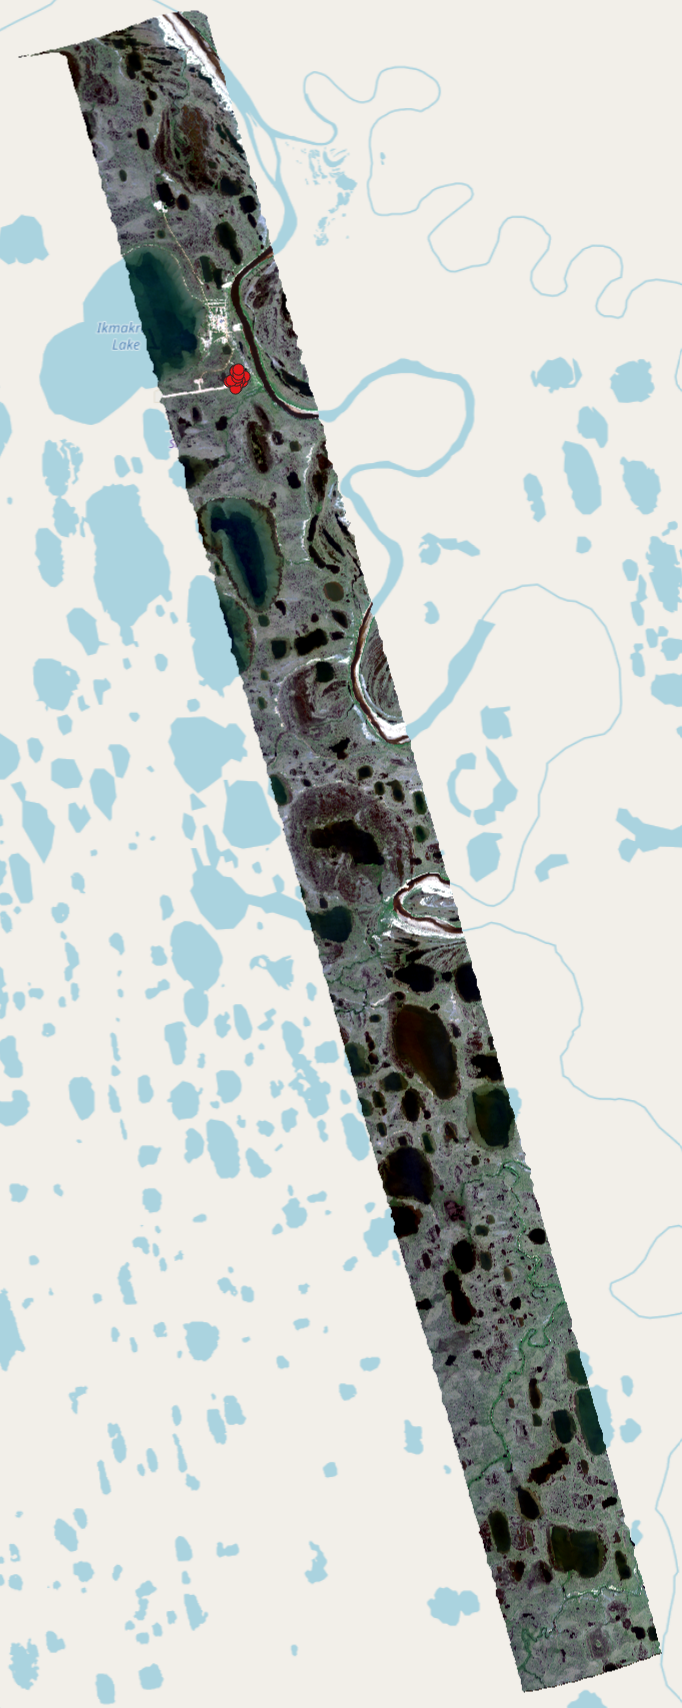
\includegraphics{\%5Bpath/to/image1.png\%5D(https://github.com/patrickangst/UWW200_Master_Thesis_public/blob/main/images/rgb.png)}
&
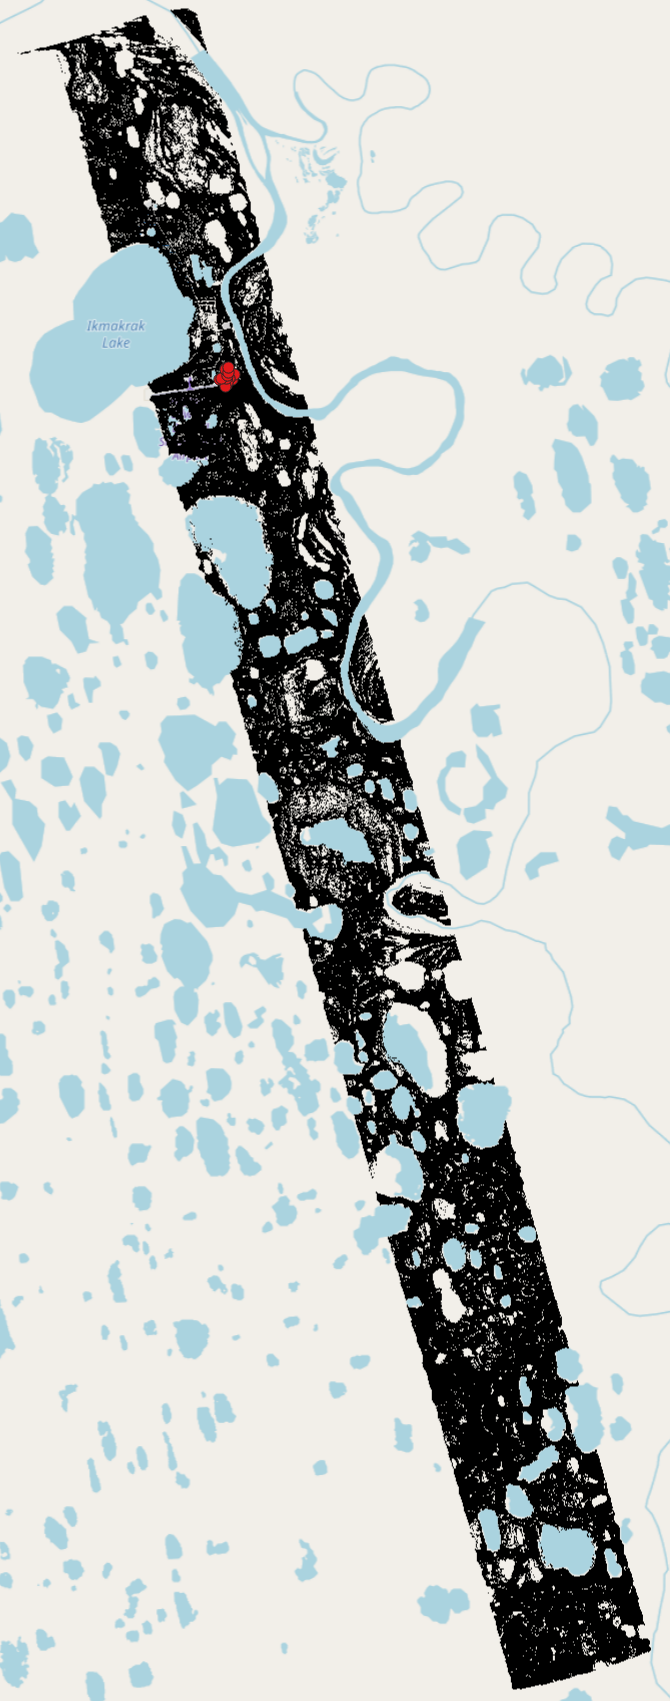
\includegraphics{\%5Bpath/to/image2.png\%5D(https://github.com/patrickangst/UWW200_Master_Thesis_public/blob/main/images/savi.png)} \\
\end{longtable}

\end{document}
